\documentclass[12pt]{article}
\usepackage[english]{babel}
\usepackage{natbib}
\usepackage{url}
\usepackage[utf8x]{inputenc}
\usepackage{amsmath}
\usepackage{graphicx}
\graphicspath{{img/}}
\usepackage{listings}
\usepackage{url}
\usepackage{parskip}
\usepackage{fancyhdr}
\usepackage{vmargin}
\setmarginsrb{3 cm}{2.5 cm}{3 cm}{2.5 cm}{1 cm}{1.5 cm}{1 cm}{1.5 cm}

\title{Lab Report on \\Image Enhancement Techniques.}								% Title
\author{Rabi Raj Khadka}								% Author
\date{June 27, 2017}											% Date


\makeatletter
\let\thetitle\@title
\let\theauthor\@author
\let\thedate\@date
\makeatother

\pagestyle{fancy}
\fancyhf{}
\rhead{\theauthor}
\lhead{\thetitle}
\cfoot{\thepage}

\begin{document}
\begin{titlepage}
	\centering
   % \vspace*{0.5 cm}
    
\includegraphics[scale = 0.3]{kheclogo.jpg}\\[1.0 cm]	% University Logo
    \textsc{\LARGE Khwopa Engineering College}\\[1.5 cm]	% University Name
	\textsc{\Large Course Code :BEG 475 IP}\\[0.5 cm]				% Course Code
	\textsc{\large Image Processing and Pattern recogntiion}\\[0.5 cm]				% Course Name
	\rule{\linewidth}{0.2 mm} \\[0.4 cm]
	{ \huge \bfseries \thetitle}\\
	\rule{\linewidth}{0.2 mm} \\[1.0 cm]
	
	% \texttt{Lab Report \#1}
	
	\rule{\linewidth}{0 mm} \\[1.0 cm]

	\begin{minipage}{0.4\textwidth}
		\begin{flushleft} \large
			\emph{Author:}\\
			\theauthor
			\end{flushleft}
			\end{minipage}~
			\begin{minipage}{0.4\textwidth}
			\begin{flushright} \large
			\emph{Roll  Number:} \\
			700324									% Your Student Number
		\end{flushright}
	\end{minipage}\\[2cm]
	
	{\large \thedate}\\[2 cm]
 
	\vfill
	
\end{titlepage}
\tableofcontents
\pagebreak
\section{Theory}
\subsection{Histogram Equalization}
Histogram equalization is the technique to change the histogram through the use of certain function into a histogram that is constant for a bright value. The probability of occurrence of gray level in an image is approximated by \\
$$P(r_k) = \frac{n_k}{N}$$  for k=0,1,2...L-1 \\
The discrete version of transformation is\\
$$ S_k = T(r_k) = \sum_{j=0}^k P_r(r_j) =  \sum_{j=1}^k\frac{n_j}{N}$$ for k=0,1,2,....L-1\\


Histogram equalization has  a disadvantage that it can generate only one type of output image. But with histogram specification, it can specify the shape of histogram that we wish the output image to have.It does not have to be uniform histogram.
\subsection{Histogram Specification}
\texttt{ Process for Histogram specification}
\begin{enumerate}
\item Obtain the transformation function T(r) by calculating the histogram equalized on the input image 
$$ S = T(r) = \sum_{j=0}^r P_r(r_j) $$
\item Obtain the transformation function G(z) by calculating the histogram equalization of desired image 
$$ Z = G(z) = \sum_{i=0}^z P_z(r_i) $$
\item Obtain the inverse transformation function $G^{-1}$\\
$$Z= G^{-1}(S) = G^{-1}[t(r)]$$
\item Obtain output image by applying the processed gray level from the inverse transformation function to all the pixels in the image.
\end{enumerate}
\subsection{Algorithm for Histogram Specification}
1. Start \\
2. Read source image and reference image\\
3. Break down the picture elements R, G, B of both color image and reference image\\
4. Make a histogram of each of the picture elements of the reference image\\
5. Assign the equalized histogram of the individual picture elements of the source image with reference to the histogram of the reference image\\
6. Merge the individual resultant individual picture elements to another variable ' histsp'  as $$ histsp(:,:,1) = outr; $$ $$ histsp(:,:,2) = outg; $$ $$ histsp(:,:,3) = outb; $$
7. show the specialized image 'histsp'\\
8. Stop
\pagebreak
\section{Code Description}
myimage = imread('\path{C\:\Users\rabiraj\Desktop\seventhsemester\ImageProcessingLab\img\one.jpg}');\\
reference = imread('\path{C\:\Users\rabiraj\Desktop\seventhsemester\ImageProcessingLab\img\two.jpg}');\\
myimage\_R=myimage(:,:,1);myimage\_G=myimage(:,:,2);myimage\_B=myimage(:,:,3);\\
reference\_R=reference(:,:,1);reference\_G=reference(:,:,2);reference\_B=reference(:,:,3);\\
hist\_myimage\_R=imhist(myimage\_R);\\
hist\_myimage\_G=imhist(myimage\_G);hist\_myimage\_B=imhist(myimage\_B);\\
hist\_reference\_R=imhist(reference\_R);\\
hist\_reference\_G=imhist(reference\_G);hist\_reference\_B=imhist(reference\_B);\\
outr =histeq(myimage\_R,hist\_reference\_R);\\
outg=histeq(myimage\_G,hist\_reference\_G);outb=histeq(myimage\_B,hist\_reference\_B);\\
histsp(:,:,1)=outr;histsp(:,:,2)=outg;histsp(:,:,3)=outb;\\
img\_lowcontrast=imadjust(rgb2gray(myimage),[0.0,1.0],[0.3,0.6]);  \\
img\_equalization = histeq(rgb2gray(myimage));\\
figure;\\
subplot(2,3,1);imshow(myimage);title('Original');\\
subplot(2,3,4);imhist(rgb2gray(myimage));title('original histogram');\\
subplot(2,3,2);imshow(img\_lowcontrast);title('lowcontrast image');\\
subplot(2,3,5);imhist(img\_lowcontrast);title('lowcontrast histogram');\\
subplot(2,3,3);imshow(img\_equalization);title('Equalized Image');\\
subplot(2,3,6);imhist(img\_equalization);title('Equalized histogram');\\
figure;\\
subplot(1,3,1);imshow(myimage);title('Original Image');\\
subplot(1,3,2);imshow(reference);title('Reference image');\\
subplot(1,3,3);imshow(histsp);title('Output Image');\\
figure;\\
subplot(3,3,1);plot(hist\_myimage\_R);title('Red Input');\\
subplot(3,3,2);plot(hist\_myimage\_G);title('Green Input');\\
subplot(3,3,3);plot(hist\_myimage\_B);title('Blue Input');\\
subplot(3,3,4);plot(hist\_reference\_R);title('Red Reference');\\
subplot(3,3,5);plot(hist\_reference\_G);title('Green Reference');\\
subplot(3,3,6);plot(hist\_reference\_B);title('Blue Reference');\\
subplot(3,3,7);plot(imhist(outr));title('output R');\\
subplot(3,3,8);plot(imhist(outg));title('output G');\\
subplot(3,3,9);plot(imhist(outb));title('output B');
%\lstinputlisting[language=Matlab]{labfive.m}
\pagebreak
\section{Result and Discussion}
The histogram of an image can be adjusted as per the user requirement. IN the image we have used, the point to be stretched is calculated by dividing the current positions of the begin and end point of the histogram by 255. By this we can adjust/stretch the image histogram. The histogram of the image can also equalized using the histeq() function\\

The histogram of one image is specified / merged with another image to form a specific image. The merged image of the first image and second image can be seen in the third one as in the output Figure 2.\\

\emph{Outputs}

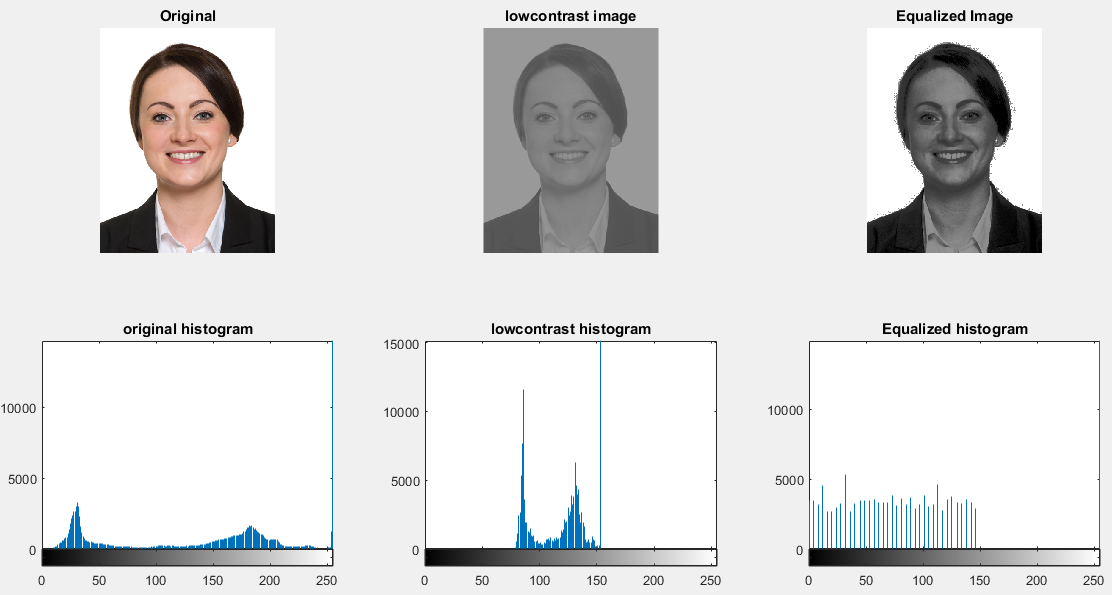
\includegraphics[scale = 0.6]{output_labfive_1.png}\\
{\centering
\texttt{Figure 1:  Equalized Specification and its Histogram}\par}
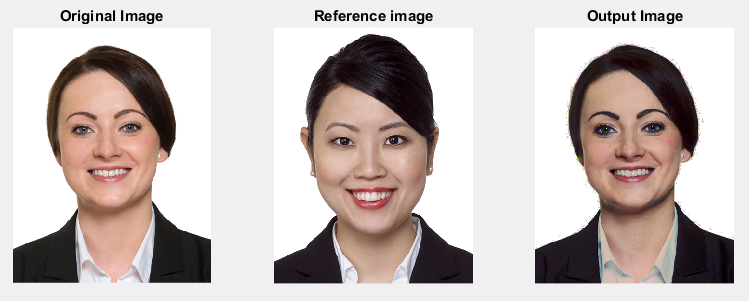
\includegraphics[scale = 0.6]{output_labfive_2.png}\\
{\centering
\texttt{Figure 2:  Histogram Specification of two image}\par}
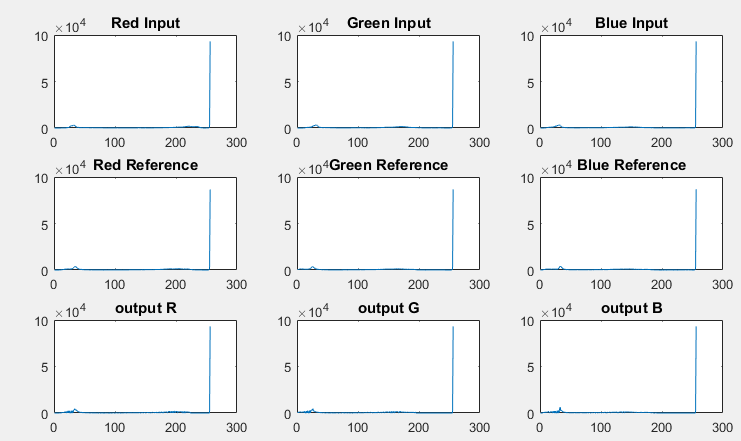
\includegraphics[scale = 0.6]{output_labfive_3.png}\\
{\centering
\texttt{Figure 3:  Histogram of  input images and output images used in Histogram Specification}\par}
\pagebreak
\section{Conclusion}
Hence, \\
We are familiarized with how the Histogram Stretching, Equalization and Specification of an image using the MATLAB application.
\end{document}